% !TEX root = ../thesis.tex
%
\tikzsetnextfilename{const-dos-approx-2}
%
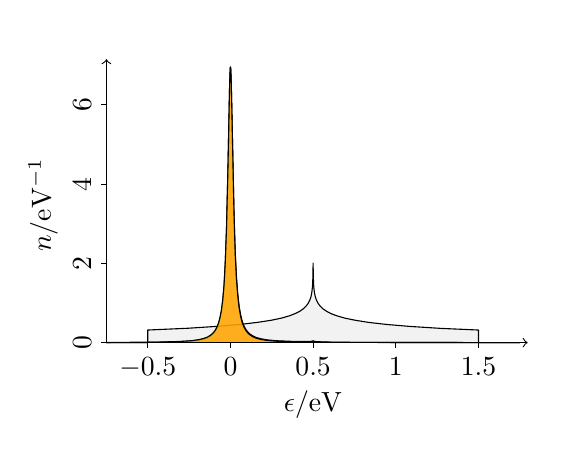
\begin{tikzpicture}[mark size=0.05cm, line cap=round]
	\draw [use as bounding box, draw=none]
		(-1.000, -1.000) rectangle +(6.750, 5.000);
	\draw [line join=round, fill opacity=0.05, fill=black] plot coordinates {
		(0.000, 0.000) (0.525, 0.000) (0.525, 0.160) (1.040, 0.183)
		(1.425, 0.208) (1.717, 0.233) (1.937, 0.260) (2.103, 0.286)
		(2.229, 0.313) (2.326, 0.341) (2.399, 0.370) (2.457, 0.399)
		(2.502, 0.431) (2.536, 0.464) (2.562, 0.499) (2.583, 0.540)
		(2.599, 0.588) (2.609, 0.640) (2.617, 0.711) (2.622, 0.823)
		(2.625, 1.010) (2.628, 0.823) (2.633, 0.711) (2.641, 0.640)
		(2.654, 0.579) (2.670, 0.534) (2.691, 0.495) (2.717, 0.461)
		(2.751, 0.429) (2.796, 0.398) (2.853, 0.368) (2.929, 0.340)
		(3.029, 0.311) (3.161, 0.284) (3.331, 0.257) (3.557, 0.231)
		(3.853, 0.206) (4.247, 0.181) (4.725, 0.160) (4.725, 0.000)
		(5.250, 0.000) };
	\draw [line join=round, fill opacity=0.7, fill=red] plot coordinates {
		(0.000, 0.000) (0.525, 0.000) (0.525, 0.004) (0.882, 0.010)
		(1.055, 0.019) (1.160, 0.031) (1.228, 0.045) (1.278, 0.062)
		(1.318, 0.083) (1.349, 0.108) (1.376, 0.138) (1.399, 0.177)
		(1.420, 0.226) (1.441, 0.298) (1.460, 0.391) (1.478, 0.531)
		(1.494, 0.714) (1.509, 0.992) (1.525, 1.424) (1.544, 2.213)
		(1.565, 3.281) (1.572, 3.483) (1.575, 3.500) (1.578, 3.490)
		(1.583, 3.392) (1.596, 2.824) (1.620, 1.674) (1.635, 1.170)
		(1.651, 0.842) (1.667, 0.628) (1.685, 0.464) (1.704, 0.356)
		(1.722, 0.281) (1.743, 0.221) (1.767, 0.174) (1.793, 0.138)
		(1.822, 0.110) (1.856, 0.087) (1.901, 0.066) (1.958, 0.050)
		(2.040, 0.035) (2.163, 0.024) (2.363, 0.016) (2.570, 0.015)
		(2.615, 0.018) (2.622, 0.021) (2.625, 0.026) (2.630, 0.019)
		(2.654, 0.014) (2.772, 0.008) (3.197, 0.003) (5.250, 0.000) };
	\draw [line join=round, fill opacity=0.6, fill=yellow] plot coordinates {
		(0.000, 0.000) (0.003, 0.002) (0.664, 0.007) (0.935, 0.015)
		(1.082, 0.025) (1.173, 0.038) (1.236, 0.053) (1.284, 0.071)
		(1.320, 0.093) (1.352, 0.120) (1.378, 0.152) (1.402, 0.194)
		(1.423, 0.248) (1.441, 0.314) (1.460, 0.409) (1.478, 0.551)
		(1.494, 0.736) (1.509, 1.017) (1.525, 1.452) (1.544, 2.240)
		(1.565, 3.294) (1.572, 3.486) (1.575, 3.500) (1.578, 3.486)
		(1.586, 3.294) (1.620, 1.644) (1.635, 1.141) (1.651, 0.817)
		(1.667, 0.605) (1.685, 0.444) (1.704, 0.337) (1.722, 0.264)
		(1.743, 0.206) (1.767, 0.160) (1.793, 0.125) (1.822, 0.099)
		(1.859, 0.075) (1.903, 0.056) (1.964, 0.040) (2.050, 0.027)
		(2.187, 0.016) (2.431, 0.008) (2.993, 0.003) (5.250, 0.000) };
	\draw [line cap=butt]
		(0.525, 0) -- +(0, -0.070) node [below] {$-0.5$}
		(1.575, 0) -- +(0, -0.070) node [below] {$0$}
		(2.625, 0) -- +(0, -0.070) node [below] {$0.5$}
		(3.675, 0) -- +(0, -0.070) node [below] {$1$}
		(4.725, 0) -- +(0, -0.070) node [below] {$1.5$}
		(0, 0.000) -- +(-0.070, 0) node [rotate=90, above] {$0$}
		(0, 1.006) -- +(-0.070, 0) node [rotate=90, above] {$2$}
		(0, 2.013) -- +(-0.070, 0) node [rotate=90, above] {$4$}
		(0, 3.019) -- +(-0.070, 0) node [rotate=90, above] {$6$};
	\draw [<->, line cap=butt]
		(5.350, 0) -- (0, 0) -- (0, 3.600);
	\node [below=\baselineskip] at (2.625, -0.070)
		{$\epsilon / \mathrm{eV}$};
	\node [rotate=90, above=\baselineskip] at (-0.070, 1.750)
		{$n / \mathrm{eV^{-1}}$};
\end{tikzpicture}%
